\documentclass[en]{../../../../../../eplexam}

\usepackage{../../../../../../eplunits}
\usepackage{../../../../../../eplcode}

\hypertitle{Programming Languages Concepts}{6}{INGI}{1131}{2011}{Janvier}
{Legat Beno\^it}
{Peter Van Roy}

\lstset{language={Oz},morekeywords={for,do,lazy}}

\section{An oscillator with a delay gate and a xor gate}
\begin{center}
  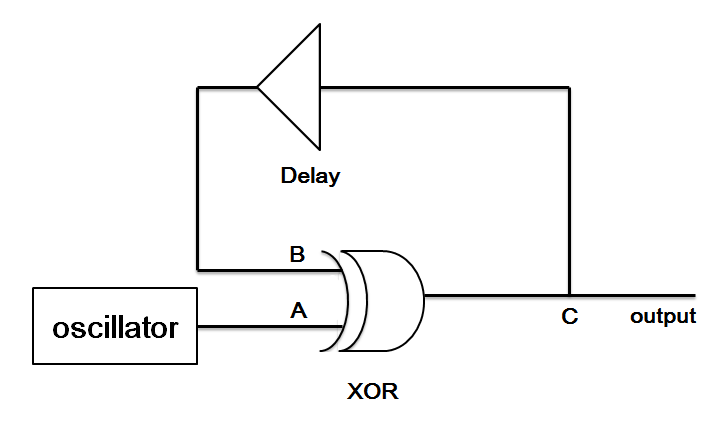
\includegraphics[width=0.6\textwidth]{circuit.png}
\end{center}
\begin{itemize}
  \item Implement each element using the simulation technique
    used in the course.
    All the elements are lazy.
  \item Give the code for the circuit shown in the figure.
  \item Show the first and second output of this circuit.
  \item Prove rigorously that the output is alternating with
    \lstinline|1| and \lstinline|0|.
    Represent the streams symbolically, for example
    A = $a_0$|$a_1$|$\cdots$,
    and analogously for B and C.
  \item Explain the lazy activations and lazy suspensions.
\end{itemize}

\section{A semi-infinite helix}
\begin{itemize}
  \item Send the message put \lstinline|(K V)| to any agent, where \lstinline|K| is a key (any atom) and \lstinline|V| is any value.
    This message will be routed to agent number \lstinline|I|, where the number \lstinline|I| is calculated as a
    deterministic function of \lstinline|K|. At that agent, the pair \lstinline|(K,V)| will be stored in a local dictionary.
  \item Send the message \lstinline|get(K X)| to any agent, where \lstinline|X| is an unbound variable. This will route
    to the agent containing the key \lstinline|K|, look up the value stored there, and bind \lstinline|X| to the value.
    If there is no value corresponding to \lstinline|K|. the special value none is returned.
\end{itemize}

\begin{solution}
  \lstinputlisting{q2.oz}
\end{solution}

\section{Building a transaction protocol}
The answer to this question is a step-by-step construction of a practical transaction protocol.

\begin{itemize}
  \item Assume that we have a naive transaction manager that gives a lock to any transaction
    that requests it, if the lock is not yet taken, and that lets a transaction release any of
    its locks whenever it wants. If another transaction has the lock, then the transaction
    manager simply asks the requesting transaction to wait. Give a scenario to show why this
    transaction manager is not serializable. Why is this undesirable ? In your answer, define
    the concept of serializability. Fix the transaction manager so that it is guaranteed to be
    serializable.
  \item What is a cascading abort ? Why is it undesirable and how can it be avoided ? Give a
    scenario to show how it can occur. Define the concepts needed to avoid it. Extend the
    transaction manager of the previous part to avoid cascading aborts.
  \item What is a deadlock ? Why is it undesirable ? Give a formal definition using the wait-for
    graph including a formal definition of the wait-for graph. What are the two kinds of nodes
    in the wait-for graph ? Give an example of deadlock in the real world (not in the world
    of transactions). Explain what is a wait-for graph in your real-world example and explain
    how the existence of deadlocks is handled there. Are they prevented or detected, and how ?
  \item Extend the transaction manager of the previous part to perform deadlock avoidance using
    transaction priorities. What are the advantages and disadvantages of this approach ?
\end{itemize}

\end{document}
